\documentclass[usenames,dvipsnames, 18pt, compress, aspectratio=169]{beamer}

% can be compiled by xelatex -shell-escape presentation.tex
% lualatex -shell-escape presentation.tex

\usetheme[]{metropolis}

\usepackage[utf8]{inputenc}
\usepackage[russian, english]{babel}
\usepackage{booktabs}
\usepackage[scale=2]{ccicons}
\usepackage{listings}
\usepackage{marvosym}
\usepackage{color}
\usepackage{xcolor}
\usepackage[document]{ragged2e}
\usepackage[export]{adjustbox}
\usepackage{fontawesome}
\usepackage{enumitem}
\usepackage{minted}
\usemintedstyle{tango}
\usepackage[normalem]{ulem}
\usepackage{tikz}
\usetikzlibrary{mindmap}
\usepackage{graphicx}
\usepackage{eso-pic}
\usepackage{verbatim}
\usepackage{smartdiagram}
\usesmartdiagramlibrary{additions}
\usetikzlibrary{trees}
\usepackage{datetime}

\usepackage{tcolorbox}
\usepackage{tabularx}
\usepackage{array}
\usepackage{colortbl}
\tcbuselibrary{skins}

\usetikzlibrary{shapes,arrows,positioning}
\graphicspath{{images/}}
\newfontfamily{\FA}{FontAwesome}

\definecolor{check}{rgb}{0.1,2,0.3}
\definecolor{fail}{rgb}{2,0.1,0.1}
\definecolor{question}{rgb}{0.9,0.9,0.0}

\def\twitter{{\FA \faTwitter}}
\def\github{{\FA \faGithub}}
\def\email{{\FA \faEnvelope}}
\def\check{\textcolor{check}{\FA \faCheck}}
\def\fail{\textcolor{fail}{\FA \faRemove}}
\def\question{\textcolor{question}{\FA \faSearch}}

\renewcommand{\ttdefault}{pcr}
\newfontfamily{\ttfamily}{Fira Code}

\usefonttheme{professionalfonts} % using non standard fonts for beamer
\usefonttheme{serif} % default family is serif
\usepackage{fontspec}
\setmainfont{Liberation Sans}
\newfontfamily\ExtraLight{Liberation Sans}
\newfontfamily\Light{Liberation Sans}
\newfontfamily\Book{Liberation Sans}
\newfontfamily\Medium{Liberation Sans}

\makeatletter
\newcommand\HUGE{\@setfontsize\Huge{32}{41}}
\makeatother

\newcommand\AtPagemyUpperLeft[1]{\AtPageLowerLeft{%
\put(\LenToUnit{0.85\paperwidth},\LenToUnit{0.05\paperheight}){#1}}}

\newcommand\AtPagemyUpperTop[1]{\AtPageLowerLeft{%
\put(\LenToUnit{0.42\paperwidth},\LenToUnit{0.90\paperheight}){#1}}}

\renewcommand{\ULthickness}{2.0pt}

\definecolor{links}{HTML}{0099FF}
\hypersetup{colorlinks, linkcolor=, urlcolor=links}

\setbeamerfont{section title}{family=\Book, size=\Huge, shape=\normalfont}
\setbeamerfont{frametitle}{family=\Book, size=\large, shape=\normalfont}
\setbeamerfont{title}{family=\Book, size=\Large, shape=\normalfont}
\setbeamerfont{subtitle}{size=\small}
\setbeamerfont{author}{family=\ExtraLight, size=\footnotesize}

\newdateformat{specialdate}{\twodigit{\THEDAY}-\twodigit{\THEMONTH}-\THEYEAR}

\newcommand\tikzmark[1]{%
  \tikz[overlay,remember picture] \coordinate (#1);}

\setbeamertemplate{title page}
{

  \vspace*{2.1cm}
  \begin{minipage}[b][\paperheight]{\textwidth}
  \begin{center}

    \ifx\inserttitle\@empty\else
    {{% \inserttitle is nonempty
      \raggedright%
      %\linespread{1.0}%
      \usebeamerfont{title}%
      \usebeamercolor[fg]{title}%
      %\vspace*{1.3em}
      \if@noSmallCapitals%
        \inserttitle%
      \else%
        \scshape{\color{black} \textbf{\begin{center}\inserttitle\end{center}}}%
      \fi%
      \vspace*{0.3em}
    }}
    \fi

    \vspace*{0.5em}%

    \ifx\insertsubtitle\@empty\else
    {{% \insertsubtitle is nonempty
      \usebeamerfont{subtitle}%
      \usebeamercolor[fg]{subtitle}%
      {\color{black} \insertsubtitle}%
      \vspace*{3.0em}%
    }}
    \fi

    \vspace*{1.0em}%

    \usebeamerfont{author}%
    \usebeamercolor[fg]{author}%
    {\color{black} \insertauthor}%

    \vspace*{1.5em}
    \fontsize{8pt}{10}\selectfont
    {\color{black} 12-05-2017}%

    \vfill
    \vspace*{2em}
  \end{center}
  \end{minipage}
}

\setbeamertemplate{section page}
{
  \vspace{2em}
  \centering
  \begin{minipage}{22em}
    \usebeamercolor[fg]{section title}
    \usebeamerfont{section title}
    {\color{black} \insertsectionhead\\[-1ex]}
  \end{minipage}
  \par
}

\setbeamertemplate{footline}
{
\begin{beamercolorbox}[wd=\textwidth,ht=3ex,dp=3ex,leftskip=0.3cm,rightskip=0.3cm]{structure}
  \usebeamerfont{page number in head/foot}
  \insertframenumber
\end{beamercolorbox}
}

\title{NOSQL\\ BEST PRACTICES}
\subtitle{FOR POSTGRESQL}
\date{\today}
\author{DMITRY DOLGOV}
\institute{}

\begin{document}
{
  \usebackgroundtemplate{
\includegraphics[width=\paperwidth]{template.png}}%
  \fontsize{17pt}{18}\selectfont
  \maketitle
}

\AddToShipoutPictureBG{
  \AtPagemyUpperLeft{{
\includegraphics[width=2.0cm,keepaspectratio]{logo.png}}}
}%

\setbeamertemplate{background canvas}{
\begin{tikzpicture}
    \clip (0,0) rectangle (\paperwidth,\paperheight);
    \fill[color=orange] (4cm, \paperheight-6pt) rectangle (\paperwidth-4cm,\paperheight);
\end{tikzpicture}
}

\fontsize{17pt}{18}\selectfont

\begin{frame}
    \frametitle{}
    \begin{center}
    \textbf{Introduction}

        \begin{itemize}[label={}]
            \item Less benchmarks
            \item More opinionated best practices
        \end{itemize}

    \end{center}
\end{frame}

\begin{frame}
    \frametitle{}
    \begin{center}
    \textbf{Introduction}

        \begin{itemize}[label={}]
            \item Application developers
            \item DBAs
            \item Extension developers
        \end{itemize}

    \end{center}
\end{frame}

\fontsize{13pt}{14}\selectfont
\section{Application developers}
\fontsize{17pt}{18}\selectfont

\begin{frame}
    \frametitle{}
    \begin{center}
    \textbf{When jsonb?}
        \begin{itemize}
            \item <+->
        \end{itemize}

        \begin{itemize}[label={\MVRightarrow}]
            \item <+-> You have a distinct flexible model
            \item <+-> You need to work with data provided in document oriented format
            \item <+-> Workaround for technical issues (large number of tables or expensive alignment)
        \end{itemize}

    \end{center}
\end{frame}
\note{
    technical reasons - Because of some performance issues you want to keep
    number of relations as small as possible (so, you denormalize some data),
    or you're playing with alignment
}

\begin{frame}
    \frametitle{}
    \begin{center}
    \textbf{When not jsonb?}
        \begin{itemize}
            \item <+->
        \end{itemize}

        \begin{itemize}[label={\MVRightarrow}]
            \item <+-> Flexibility "just in case"
            \item <+-> Reluctance to create a migration
            \item <+-> Use jsonb column as a "garbage can"
        \end{itemize}

    \end{center}
\end{frame}

\begin{frame}
    \frametitle{}
    \begin{center}
    \textbf{Jsonb -> Relation}

        \begin{columns}[T,onlytextwidth]
        \column{0.5\textwidth}
        \begin{itemize}[leftmargin=*]
            \item 
\includegraphics[width=6cm,height=5cm]{document.jpg}
        \end{itemize}

        \column{0.5\textwidth}
        \begin{itemize}[leftmargin=*]
            \item 
\includegraphics[width=6cm,height=5cm]{relation.png}
        \end{itemize}

        \end{columns}

    \end{center}
\end{frame}

\begin{frame}
    \frametitle{}
    \begin{center}
    \textbf{When to move from jsonb to relation?}
        \begin{itemize}
            \item <+->
        \end{itemize}

        \begin{itemize}[label={\MVRightarrow}]
            \item <+-> Queries rely significantly in information about\\
                internal structure of documents
            \item <+-> There are too many constraints for documents
            \item <+-> Some parts of document are used much more\\
                frequently than other
        \end{itemize}

    \end{center}
\end{frame}

\begin{frame}
    \frametitle{}
    \begin{center}

        \inputminted[
            fontsize=\normalsize,
        ]{sql}{sql/complex_where.sql}

    \end{center}
\end{frame}

\begin{frame}
    \frametitle{}
    \begin{center}
    \textbf{Complicated conditions}

        \begin{itemize}[label={\MVRightarrow}]
            \item jsquery
            \item SQL/JSON
        \end{itemize}

    \end{center}
\end{frame}

\begin{frame}
    \frametitle{}
    \begin{center}
    \textbf{Complicated conditions}

        \inputminted[
            fontsize=\normalsize,
        ]{sql}{sql/complex_where_jsquery.sql}

    \end{center}
\end{frame}

\begin{frame}
    \frametitle{}
    \begin{center}
    \textbf{Complicated conditions}

        \inputminted[
            fontsize=\normalsize,
        ]{sql}{sql/complex_where_standard.sql}

    \end{center}
\end{frame}

\begin{frame}
    \frametitle{}
    \begin{center}
    \textbf{Complicated select}

        \inputminted[
            fontsize=\normalsize,
        ]{sql}{sql/complex_select.sql}

    \end{center}
\end{frame}

\begin{frame}
    \frametitle{}
    \begin{center}
    \textbf{Jsonb -> Relation}

        \begin{columns}[T,onlytextwidth]
        \column{0.3\textwidth}
        \begin{itemize}[leftmargin=*]
            \item 
\includegraphics[width=4cm,height=4cm]{document.jpg}
        \end{itemize}

        \column{0.3\textwidth}
        \begin{itemize}[leftmargin=*]
            \item 
\includegraphics[width=4cm,height=4cm]{schema.jpg}
        \end{itemize}

        \column{0.3\textwidth}
        \begin{itemize}[leftmargin=*]
            \item 
\includegraphics[width=4cm,height=4cm]{relation.png}
        \end{itemize}

        \end{columns}

    \end{center}
\end{frame}

\begin{frame}
    \frametitle{}
    \begin{center}
    \textbf{Constraints}

        \begin{itemize}[label={\MVRightarrow}]
            \item Simple checks for value, type or size
            \item More convenient checks with jsquery
            \item Json schema
        \end{itemize}

    \end{center}
\end{frame}

\begin{frame}
    \frametitle{}
    \begin{center}
    \textbf{Constraints}

        \begin{itemize}[label={\MVRightarrow}]
            \item Simple checks for value, type or size
            \item More convenient checks with jsquery
            \item Json schema
        \end{itemize}

    \end{center}
\end{frame}

\begin{frame}
    \frametitle{}
    \begin{center}
    \textbf{Constraints}

        \inputminted[
            fontsize=\normalsize,
        ]{sql}{sql/constraints.sql}

    \end{center}
\end{frame}

\begin{frame}
    \frametitle{}
    \begin{center}
    \textbf{Relation -> Jsonb}

        \begin{columns}[T,onlytextwidth]
        \column{0.5\textwidth}
        \begin{itemize}[leftmargin=*]
            \item 
\includegraphics[width=6cm,height=5cm]{relation.png}
        \end{itemize}

        \column{0.5\textwidth}
        \begin{itemize}[leftmargin=*]
            \item 
\includegraphics[width=6cm,height=5cm]{document.jpg}
        \end{itemize}

        \end{columns}

    \end{center}
\end{frame}

\begin{frame}
    \frametitle{}
    \begin{center}

        \inputminted[
            fontsize=\large,
        ]{sql}{sql/jsonb_agg.sql}

    \end{center}
\end{frame}

\fontsize{13pt}{14}\selectfont
\section{Seamless interaction\\ between json and relation}
\fontsize{17pt}{18}\selectfont

\fontsize{17pt}{19}\selectfont
\begin{frame}
    \frametitle{}
    \begin{center}

    \inputminted[
        fontsize=\Large,
    ]{json}{sql/with_array_data.json}

    \end{center}
\end{frame}

\fontsize{17pt}{19}\selectfont
\begin{frame}
    \frametitle{}
    \begin{center}

    \begin{overprint}
    \onslide<1>
    \inputminted[
        fontsize=\Large,
        escapeinside=||
    ]{sql}{sql/with_array.sql}

    \onslide<2>
    \inputminted[
        fontsize=\Large,
        escapeinside=||
    ]{sql}{sql/with_array_highlight.sql}
    \end{overprint}

    \inputminted[
        fontsize=\large,
    ]{bash}{sql/with_array.sh}

    \end{center}
\end{frame}

\fontsize{17pt}{19}\selectfont
\begin{frame}
    \frametitle{}
    \begin{center}

    \inputminted[
        fontsize=\Large,
    ]{json}{sql/iterate_document_data.json}

    \end{center}
\end{frame}

\fontsize{17pt}{19}\selectfont
\begin{frame}
    \frametitle{}
    \begin{center}

    \begin{overprint}
    \onslide<1>
    \inputminted[
        fontsize=\Large,
        escapeinside=||
    ]{sql}{sql/iterate_document.sql}

    \onslide<2>
    \inputminted[
        fontsize=\Large,
        escapeinside=||
        ]{sql}{sql/iterate_document_highlight.sql}
    \end{overprint}

    \inputminted[
        fontsize=\large,
    ]{bash}{sql/iterate_document.sh}

    \end{center}
\end{frame}

\begin{frame}
    \frametitle{}
    \begin{center}
    \textbf{Place for ID}

        \begin{itemize}[label={\MVRightarrow}]
            \item Inside a document
            \item As as separate column
        \end{itemize}

    \end{center}
\end{frame}

\begin{frame}
    \frametitle{}
    \begin{center}

        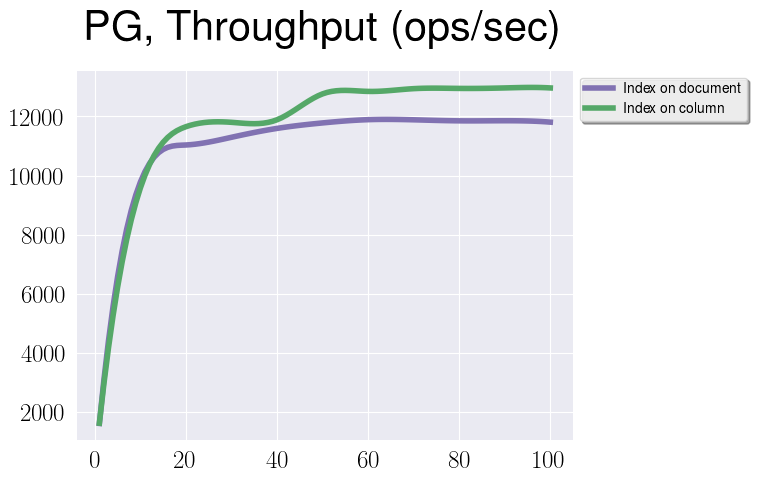
\includegraphics[width=0.75\textwidth,center]{pg_id_place.png}

    \end{center}
\end{frame}

\begin{frame}
    \frametitle{}
    \begin{center}
        \textbf{Multiple jsonb columns}

        \begin{itemize}[label={\MVRightarrow}]
            \item Keep at the end for readability
            \item tuple\_deform
        \end{itemize}

    \end{center}
\end{frame}

\begin{frame}
    \frametitle{}
    \begin{center}
    \textbf{Multiple jsonb columns}

        \vspace{1cm}
        \begin{tcolorbox}[adjusted title= Table]
        \begin{tabular}{c|c|c|c|c|c}
            \tikzmark{start} value & \tikzmark{right} value & value & value & value & value... \\\hline
        value & value & value & value & value & value... \\\hline
        \tikzmark{end} value & value & value & value & value & value...
        \end{tabular}
        \end{tcolorbox}

        \begin{tikzpicture}[overlay,remember picture]
            \draw[->, line width=1mm]
            let \p1=(start), \p2=(end) in ($(\x1,\y1)+(-1.2,0.2)$) -- node[] {} ($(\x1,\y2)+(-1.2,0.0)$);
        \end{tikzpicture}

        \begin{tikzpicture}[overlay,remember picture]
            \draw[->, line width=1mm, color=white]
            let \p1=(start), \p2=(right) in ($(\x1,\y1)+(1.5,1.3)$) -- node[] {} ($(\x1,\y2)+(12.0,1.3)$);
        \end{tikzpicture}

        \begin{tikzpicture}[overlay,remember picture]
            \draw[line width=1mm, color=red, rounded corners]
            let \p1=(start), \p2=(right) in ($(\x1,\y1)+(9.5,0.8)$) rectangle ($(\x1,\y2)+(12.0,-2.1)$);
        \end{tikzpicture}


    \end{center}
\end{frame}

\begin{frame}
    \frametitle{}
    \begin{center}
    \textbf{Multiple jsonb columns}

        \vspace{1cm}
        \begin{tcolorbox}[adjusted title= Table]
        \begin{tabular}{c|c|c|c|c|c}
        \tikzmark{start} value... & \tikzmark{right} value & value & value & value & value \\\hline
        value... & value & value & value & value & value \\\hline
        \tikzmark{end} value... & value & value & value & value & value
        \end{tabular}
        \end{tcolorbox}

        \begin{tikzpicture}[overlay,remember picture]
            \draw[->, line width=1mm]
            let \p1=(start), \p2=(end) in ($(\x1,\y1)+(-1.2,0.2)$) -- node[] {} ($(\x1,\y2)+(-1.2,0.0)$);
        \end{tikzpicture}

        \begin{tikzpicture}[overlay,remember picture]
            \draw[->, line width=1mm, color=white]
            let \p1=(start), \p2=(right) in ($(\x1,\y1)+(1.5,1.3)$) -- node[] {} ($(\x1,\y2)+(12.0,1.3)$);
        \end{tikzpicture}

        \begin{tikzpicture}[overlay,remember picture]
            \draw[line width=1mm, color=red, rounded corners]
            let \p1=(start), \p2=(right) in ($(\x1,\y1)+(-0.3,0.8)$) rectangle ($(\x1,\y2)+(2.3,-2.1)$);
        \end{tikzpicture}

    \end{center}
\end{frame}

\fontsize{17pt}{18}\selectfont
\begin{frame}
  \vspace*{2.5cm}
  \begin{minipage}[b][\paperheight]{\textwidth}
  \begin{center}

      %\raggedright%
      \linespread{1.0}%
      \usebeamerfont{title}%
      \usebeamercolor[fg]{title}%
      \if@noSmallCapitals%
        Questions?
      \else%
        \scshape{\color{black} Questions?}%
      \fi%
      \vspace*{0.3em}

      \usebeamerfont{subtitle}%
      \fontsize{13pt}{14}\selectfont
      \usebeamercolor[fg]{subtitle}%
        \begin{itemize}[label={}]
            \item {\color{black} \github\ github.com/erthalion}
            \item {\color{black} \twitter\ @erthalion}
            \item {\color{black}\email\ 9erthalion6 at gmail dot com}
        \end{itemize}
      \vspace*{2.5em}%

    \vfill
    \vspace*{2em}
  \end{center}
  \end{minipage}

\end{frame}

\end{document}
